% !TEX root = ../thesis.tex

\chapter{Appendix to Robust shattering}


\section{Additional dualities}
\label{app:face-DWs}

\begin{figure}
    \centering
    \includegraphics[width=0.3\linewidth]{img/signs2.pdf}
    \caption[The sign convention that we introduce to define domain wall variables]{The sign convention that we introduce to define domain wall variables of the form $\hat{Z}^\dagger_i Z^{\phantom{\dagger}}_j$ living on faces, which correspond to domain walls amongst even sublattice spins and amongst odd sublattice spins. Vertices that contribute a $Z$ ($Z^\dagger$) to the domain wall degree of freedom on a given face are denoted by red (blue) shaded regions. This choice affects the local constraints that any domain wall configuration must satisfy.}
    \label{fig:sign-convention}
\end{figure}

Here, we describe a further duality of the two-dimensional models~\eqref{eqn:four-spin-flip} and~\eqref{eqn:QF-dual}, which involves introducing two degrees of freedom per face that correspond to domain wall variables between spins belonging to the same sublattice.
That is, a spin situated at a vertex with coordinates $(x,y)$ belongs to the even (odd) sublattice if $x+y$ is even (odd).
The introduction of these new degrees of freedom is motivated by Eq.~\eqref{eqn:vertex-constraint-operator}, which requires that, around a given face, the two spins on the even sublattice must match, or the two spins on the odd sublattice must match (or both).
Explicitly, given four vertices around a face, $v_1$, $v_2$, $v_3$, and $v_4$ (no ordering implied), with $v_1$, $v_3$ belonging to the even sublattice, and $v_2$, $v_4$ to the odd sublattice, we construct domain wall variables $\hat{\tau}_{f,+}^{z} = \hat{{Z}}_{v_1}^\dagger \hat{{Z}}_{v_3}^{\phantom{\dagger}}$ and $\hat{\tau}_{f,-}^z = \hat{{Z}}_{v_2}^\dagger \hat{{Z}}_{v_4}^{\phantom{\dagger}}$.
In this language, the constraint is particularly simple: On any face $f$, domain walls (defined by ${\tau}_{f,s}^z \neq 1$) cannot intersect. 

For $m>2$, the $\hat{Z}_v$ operators are not Hermitian, so there exists a choice in which $\hat{Z}$ operators are conjugated. Illustrating those vertices that contribute a $\hat{Z}$ ($\hat{Z}^\dagger$) by red (blue) shaded regions, the convention that we utilize is illustrated in Fig.~\ref{fig:sign-convention}.
In principle, there are $m-1$ species of domain wall per sublattice. However, when illustrating spin configurations we choose not to distinguish between domain walls on the even and odd sublattices. The configurations on faces for $m=3$ consistent with the constraint are:
%
\begin{equation*}
    \underset{ (0,\,0) }{%
    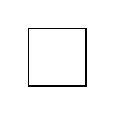
\begin{tikzpicture}[baseline={(0,-0.12)}, scale=1]
        \draw [semithick] (-2.4ex, -2.4ex) rectangle (2.4ex, 2.4ex);
        \begin{scope}[every node/.style={minimum size=0mm, inner sep=0}]
            \node (A) at (-2.4ex, -2.4ex) {};
            \node (B) at (-2.4ex, 2.4ex) {};
            \node (C) at (2.4ex, 2.4ex) {};
            \node (C) at (2.4ex, -2.4ex) {};
        \end{scope} 
    \end{tikzpicture}}
    \qquad
    \underset{ (1,\, 0) }{%
    \begin{tikzpicture}[baseline={(0,-0.12)}, scale=1]
        \draw [semithick] (-2.4ex, -2.4ex) rectangle (2.4ex, 2.4ex);
        \begin{scope}[every node/.style={minimum size=0mm, inner sep=0}]
            \node (A) at (-2.4ex, -2.4ex) {};
            \node (B) at (-2.4ex, 2.4ex) {};
            \node (C) at (2.4ex, 2.4ex) {};
            \node (D) at (2.4ex, -2.4ex) {};
        \end{scope}
        \begin{scope}[on background layer]
            \draw [ultra thick, DarkerBlue] (A) -- (C);
        \end{scope}
    \end{tikzpicture}}
    \quad
    \underset{ (0,\, 1) }{%
    \begin{tikzpicture}[baseline={(0,-0.12)}, scale=1]
        \draw [semithick] (-2.4ex, -2.4ex) rectangle (2.4ex, 2.4ex);
        \begin{scope}[every node/.style={minimum size=0mm, inner sep=0}]
            \node (A) at (-2.4ex, -2.4ex) {};
            \node (B) at (-2.4ex, 2.4ex) {};
            \node (C) at (2.4ex, 2.4ex) {};
            \node (D) at (2.4ex, -2.4ex) {};
        \end{scope}
        \begin{scope}[on background layer]
            \draw [ultra thick, DarkerBlue] (B) -- (D);
        \end{scope}
    \end{tikzpicture}}
    \qquad
    \underset{ (2,\, 0) }{%
    \begin{tikzpicture}[baseline={(0,-0.12)}, scale=1]
        \draw [semithick] (-2.4ex, -2.4ex) rectangle (2.4ex, 2.4ex);
        \begin{scope}[every node/.style={minimum size=0mm, inner sep=0}]
            \node (A) at (-2.4ex, -2.4ex) {};
            \node (B) at (-2.4ex, 2.4ex) {};
            \node (C) at (2.4ex, 2.4ex) {};
            \node (D) at (2.4ex, -2.4ex) {};
        \end{scope}
        \begin{scope}[on background layer]
            \draw [ultra thick, LighterBlue] (A) -- (C);
        \end{scope}
    \end{tikzpicture}}
    \quad
    \underset{ (0,\, 2) }{%
    \begin{tikzpicture}[baseline={(0,-0.12)}, scale=1]
        \draw [semithick] (-2.4ex, -2.4ex) rectangle (2.4ex, 2.4ex);
        \begin{scope}[every node/.style={minimum size=0mm, inner sep=0}]
            \node (A) at (-2.4ex, -2.4ex) {};
            \node (B) at (-2.4ex, 2.4ex) {};
            \node (C) at (2.4ex, 2.4ex) {};
            \node (D) at (2.4ex, -2.4ex) {};
        \end{scope}
        \begin{scope}[on background layer]
            \draw [ultra thick, LighterBlue] (B) -- (D);
        \end{scope}
    \end{tikzpicture}}
\end{equation*}
%
%
where the labels denote $(\alpha_{f,+}, \alpha_{f,-})$ assuming the top left and bottom right vertices belong to the even sublattice (for a given face and sublattice, $\alpha$ is defined by ${\tau}^z = e^{2\pi i \alpha / m}$).
The convention in Fig.~\ref{fig:sign-convention} enforces constraints on the colors of domain walls on adjacent faces.
Namely, the domain wall variables on the four faces around a vertex $v$, belonging to sublattice $s$, satisfy $\prod_{f \in v} \hat{\tau}^z_{f,-s} = \mathds{1}$, equivalent to $\sum_{f\in v} \alpha_{f,-s} = 0 \mod m$. Graphically, a domain wall will therefore change color at every vertex, unless it branches or meets another domain wall (at a vertex), as shown in Fig.~\ref{subfig:random-face}.

%%%%%%%%%%%%%%%%%%%%%%%%%%%%%%%%%%%%%%%%%%%%%%%%%%%%%%%%%%%%%%%%%%%%%%%%%%%%%%%%
%%%%%%%%%%%%%%%%%%%%%%%%%%%%%%%%%%%%%%%%%%%%%%%%%%%%%%%%%%%%%%%%%%%%%%%%%%%%%%%%
%%%%%%%%%%%%%%%%%%%%%%%%%%%%%%%%%%%%%%%%%%%%%%%%%%%%%%%%%%%%%%%%%%%%%%%%%%%%%%%%

\section{Enumerating sectors and frozen states}
\label{app:enumeration}


%------------------------------------------------------------------------------%
%------------------------------------------------------------------------------%
%------------------------------------------------------------------------------%

\subsection{Krylov sectors in the pair-flip model}

The Bethe lattice mapping presented in Fig.~\ref{fig:Bethe} can also be applied in 1D to facilitate the counting of labels and Krylov sector dimensions~\cite{Caha2018PairFlip,Moudgalya2022Commutant}.
The `final' position on the Bethe lattice after traversing the entire system from left to right, having begun at the root node of the Bethe lattice, is in one-to-one correspondence with the label introduced in Sec.~\ref{sec:1D-pair-flip}, which identifies distinct Krylov sectors in the 1D pair-flip model with open boundaries. Similarly, each walk is in one-to-one correspondence with a spin configuration.
Hence, the number of spin configurations that map to the same label (with length $\ell$) is equal to the number of walks of length $L$ that reach a given point with depth $\ell$ on the Bethe lattice (note that this number will depend only on $\ell$).
The number of such walks $G_L^{(\ell)}$ -- equal to the dimension of the Krylov sector for a label of length $\ell$ -- is enumerated by the generating functions found in Refs.~\cite{Hart2020GFs,Caha2018PairFlip}: 
%
%
\begin{equation}
    G^{(\ell)}(x) = \sum_{L=0}^{\infty} G_L^{(\ell)} x^L = \left( \frac{1-\sqrt{1-4(m-1)x^2}}{2(m-1)x} \right)^\ell \frac{2(m-1)}{m-2+m\sqrt{1-4(m-1)x^2}}
    \, .
    \label{eqn:GF}
\end{equation}
%
%
Note that $G^{(\ell)}(x)$ enforces that $G_L^{(\ell)} = 0$ if $\ell$ and $L$ have opposite parity, as is required. The number of sites on the Bethe lattice that are accessible after $L$ steps is given by Eq.~\eqref{eqn:unique-labels}. The exponential growth the Krylov sector dimension $G_L^{(\ell)}$ is determined directly (up to subexponential factors) by the radius of convergence of~Eq.~\eqref{eqn:GF}~\cite{Flajolet2009Combinatorics}. Specifically, we have
%
%
\begin{equation}
    G_L^{(\ell)} \sim (2\sqrt{m-1})^L
    \label{eqn:Krylov-growth}
\end{equation}
%
%
as $L \to \infty$ for fixed $\ell$.
Insight into the subexponential factors can be obtained by performing a singularity analysis of Eq.~\eqref{eqn:GF}~\cite{Flajolet1990Singularity, Flajolet2009Combinatorics, Caha2018PairFlip}. Expanding around the singularities at $x = \pm 2\sqrt{m-1}$, we find that
%
%
\begin{equation}   
    G_L^{(\ell)} = 2\left( \ell + \frac{m}{m-2} \right) \frac{m-1}{m-2} \sqrt{\frac{2}{\pi L^3}} 2^L \sqrt{m-1}^{L-\ell} \left[ 1 + \cal{O}(L^{-1}) \right]
    \, ,
\end{equation}
%
%
as $L \to \infty$ for fixed, $\cal{O}(1)$ values of $\ell$. 
This result shows that, at least for $m > 2$, sectors with larger label lengths $\ell$ are exponentially suppressed in size with respect to the $\ell = 0$ sector.
Additionally, we can deduce that no Krylov sector grows faster than $(2\sqrt{m-1})^L$ as $L \to \infty$.

We can also write down a generating function that counts the number of labels belonging to each \emph{symmetry sector}. That is, using this generating function, we can deduce into how many Krylov sectors a particular symmetry sector decomposes.
To do this, we must account for the $\text{U}(1)$ charges associated with each of the $m$ colors. Let the generating variables $\mathbf{y} = \{ y_\alpha \}$ keep track of the charge $N^\alpha$ defined in Eq.~\eqref{eqn:PF-symmetry}. Restricting to $m=3$ for simplicity, we can then introduce the two transfer matrices [the row (column) index corresponds to the current (previous) step]
%
%
\begin{equation}
    T_\sigma = 
    x
    \begin{pmatrix}
        0 & y_r^{\sigma} & y_r^{\sigma} \\
        y_g^{\sigma} & 0 & y_g^{\sigma} \\
        y_b^{\sigma} & y_b^{\sigma} & 0
    \end{pmatrix}
    \, ,
\end{equation}
%
%
with $\sigma = \pm 1$. More generally, the transfer matrix will be an $m\times m$ matrix with the above structure; the zeros along the diagonal enforce that the color of a given dot cannot match the color of the previous dot in the label. The sign $\sigma$ corresponds to whether an even or an odd edge is being traversed, which add to or subtract from the corresponding $\text{U}(1)$ charge.
The generating variable $x$ records the length of the label.
For open boundary conditions, the full generating function admits the expansion 
%
%
\begin{equation}
    F(x; \mathbf{y} ) = 1 + \sum_{i=1}^{m} \left( T_0 + T_- T_0 + T_+T_- T_0 + T_-T_+T_-T_0 + \dots \right)_i
    \, ,
\end{equation}
%
%
where the initial condition $T_0 = x(y_r, y_g, y_b)^T$ corresponds to the first (unconstrained) dot, which we assume belongs to the even sublattice.
In the presence of periodic boundaries, an analogous expression can be obtained by removing the initial condition $T_0$ and replacing the sum over $i$ by a trace.
Factoring out the repeating combination $T_+ T_-$, we find that
%
%
\begin{subequations}
\begin{align}
    F(x; \mathbf{y} ) &= 1 + \sum_{i=1}^m \sum_{\ell=1}^{\infty} [(\mathds{1}+T_-)(T_+T_-)^{\ell - 1}T_0]_{i}  \\
                      &= 1 + \sum_{i=1}^m [(\mathds{1}+T_-)(\mathds{1}-T_+T_-)^{-1} T_0]_{i} \label{eqn:U(1)-GF-matrixinverse}
                      \, .
\end{align}%
\end{subequations}
%
%
where we used $\sum_{n=0}^\infty A^n = (\mathds{1} - A)^{-1}$, which is convergent if the spectral radius of the matrix $A$ is strictly less than unity. 
The matrix inverse in Eq.~\eqref{eqn:U(1)-GF-matrixinverse} can be evaluated exactly to arrive at the expression
%
%
\begin{equation}
      F(x; \mathbf{y} ) = \frac{\left(1-x^2\right) \left[ 1 + x (y_r+y_g+y_b)+2x^2\right]}{1+x^2+4 x^4  - x^2 \left[\frac{y_r}{y_g}+\frac{y_r}{y_b} + \frac{y_g}{y_b}+\frac{y_g}{y_r} + \frac{y_b}{y_r} + \frac{y_b}{y_g}\right]}
      \, .
\end{equation}
%
%
As required, throwing away the information about the $\text{U}(1)$ charges reduces to $F(x; \mathbf{1}) = (1+x)/(1-2x)$, with coefficients $3 \times 2^{n-1}$ for $n \geq 1$, equal to the total number of labels of length $n$. Performing the same procedure for case $m=2$ provides another simple example:
%
%
\begin{equation}
    \frac{y_r y_b\left(1-x^2\right)  \left[ 1+x (y_r+y_b) + x^2\right]}{ \left(x^2 y_r-y_b\right) \left(x^2 y_b-y_r\right) } = 
    1+\sum_{n=1}^{\infty} \frac{y_r^n + y_b^n}{(y_r y_b)^{\lfloor n/2 \rfloor}} x^n
    \, ,
\end{equation}
%
%
since there is only one label associated with each symmetry sector.

Returning to $m=3$, let us evaluate the total number of labels that live in the symmetry sector with vanishing charge for all three colors, $N^\alpha = 0$.
Such ``uncharged'' labels are also useful for constructing labels of arbitrary length compatible with a given set of symmetry quantum numbers: Given a label belonging to the appropriate sector, an uncharged label can be appended or prepended (subject to the constraint that neighbors may not match) to produce new labels belonging to the same sector.
To extract the generating function of uncharged labels, we are required to evaluate the integral
%
%
\begin{equation}
    \int_{-\pi}^{\pi} \frac{\mathrm{d}\phi_r \mathrm{d}\phi_g \mathrm{d}\phi_b}{(2\pi)^3}  \frac{\left(1-x^2\right) \left[ 1 + x (e^{i\phi_r}+e^{i\phi_g}+e^{i\phi_b})+2x^2\right]}{1+x^2+4 x^4  - 2x^2 \left[\cos(\phi_r - \phi_g)+\cos(\phi_g - \phi_b) + \cos(\phi_b - \phi_r)\right]}
    \, .
\end{equation}
%
%
The number of labels belonging to other symmetry sectors can be obtained similarly by first multiplying by $\exp(-i \sum_\alpha \phi_\alpha N^\alpha )$.
We can make progress by shifting (say) $\phi_{g,b} \to \phi_{g,b} + \phi_r$, making the integral over $\phi_r$ trivial. Additionally, we define the function $E(x) = (1+x^2+4x^4)/x^2$ and restructure the trigonometric functions, which brings the integral into the form
%
%
\begin{equation}
    \frac{\left(1-x^2\right) ( 1+2x^2)}{x^2}\int_{-\pi}^{\pi} \frac{ \mathrm{d}k_1 \mathrm{d}k_2}{(2\pi)^2}  \frac{1}{E(x) - 2\left[\cos( k_1) + 2 \cos(\frac{k_1}{2})\cos(\frac{k_1}{2}-k_2)\right]}
    \, .
 \end{equation}
%
%
This integral is equal to the Green's function of a single tight-binding quantum particle hopping on a triangular lattice~\cite{Horiguchi1972Lattice}, for which (in appropriate coordinates) the dispersion relation may be written $E(\mathbf{k}) = 2\left[\cos( k_1) + 2 \cos(\frac{k_1}{2})\cos(\frac{k_1}{2}-k_2)\right]$. We can therefore write down an exact expression for the generating function of uncharged configurations
%
%
\begin{equation}
    F_0(x) \equiv [y_r^0 y_g^0 y_b^0]F(x; \mathbf{y}) = \frac{2\left(1-x^2\right) ( 1+2x^2)}{\pi x^2 (\lambda-1)^{3/2} (\lambda+3)^{1/2}}  K\left( \frac{4\lambda^{1/2}}{(\lambda-1)^{3/2} (\lambda+3)^{1/2}} \right) 
    \, ,
    \label{eqn:neutral-labels-exact}
\end{equation}
%
%
where $K(x)$ is the complete elliptic integral of the first kind and we have introduced $\lambda(x) = \sqrt{3+E(x)}$. The first few pattern lengths that belong to the uncharged symmetry sector that derive from Eq.~\eqref{eqn:neutral-labels-exact} are
%
%
\begin{equation}
    F_0(x) = 1+6 x^6+6 x^8+42 x^{10}+120 x^{12}+426 x^{14}+\dots
\end{equation}
%
%
The shortest uncharged pattern has length six and corresponds to a three-dot pattern repeated twice, such as
$\left\lvert\kern1pt%
\begin{tikzpicture}[baseline={(0,-0.12)},x=2.4ex, y=2.4ex]
        \dualRcirc{0}{0};
        \dualGcirc{1}{0};
        \dualBcirc{2}{0};
        \dualRcirc{3}{0};
        \dualGcirc{4}{0};
        \dualBcirc{5}{0};
\end{tikzpicture}\kern1pt\right\rangle$.
The six labels of length $\ell = 8$ are the same six labels as $\ell = 6$ surrounded by the unique color that is not equal to the first or last color in the corresponding $\ell=6$ label.
Asymptotically, the number of patterns of length $\ell$ within the uncharged symmetry sector scales (up to polynomial corrections) as $\sim 2^\ell$.

\begin{figure}[th!]
    \centering
    \includegraphics[width=0.55\linewidth]{img/exact_distribution.pdf}
    \caption[Exact distribution of Krylov sectors in the pair-flip model]{Exact distribution of Krylov sectors in the uncharged symmetry sector, obtained from the generating functions~\eqref{eqn:GF} and~\eqref{eqn:neutral-labels-exact}. $P(\ell)$ is the probability that a state drawn at random from the uncharged symmetry sector with uniform probability belongs to a Krylov sector corresponding to label length $\ell$. The largest Krylov sector, which corresponds to label length $\ell = 0$, represents a vanishingly small fraction of the symmetry sector.}
    \label{fig:krylov-distribution}
\end{figure}

Lastly, we note that fragmentation in the PF model is \emph{strong}~\cite{Khemani2020Localization, Sala2020Fragmentation}: In the thermodynamic limit, an arbitrary state chosen from any fixed symmetry sector (i.e., one whose charge does not scale with $L$) belongs to that sector's largest Krylov sector with probability zero. To see this, recall that any symmetry sector has a minimal length $L_\text{min}$ on which it exists. To bound the size of the symmetry sector, we can then place any uncharged spin configuration on the remainder of the system. For $m=3$ and systems of length $L=L_\text{min}+6n$, we can place $n$ red spins, $n$ blue spins, and $n$ green spins on the even sublattice (and similarly for the odd sublattice), giving 
%
%
\begin{equation}
    D^\text{sym}_0 > {\left[ \frac{(3n)!}{(n!)^3} \right]}^2 \sim \frac{3^{6 n+1}}{4 \pi ^2 n^2}
\end{equation}
%
%
uncharged spin configurations.
Hence, every fixed symmetry sector has a dimension that scales asymptotically as $\sim 3^{L-L_\text{min}}$ up to polynomial corrections, while no Krylov sector grows faster than $\sim (2\sqrt{2})^L$~\eqref{eqn:Krylov-growth}.  
For larger $m$, symmetry sectors contain $\sim m^L$ states, while no Krylov sector grows faster than $\sim(2\sqrt{m-1})^L$.
This result is illustrated for the uncharged symmetry sector in Fig.~\ref{fig:krylov-distribution}, which shows that an arbitrary state is most likely to belong to a Krylov sector of intermediate size, and that the probability of belonging to any particular Krylov sector vanishes in the thermodynamic limit.

%------------------------------------------------------------------------------%
%------------------------------------------------------------------------------%
%------------------------------------------------------------------------------%

\subsection{Labels in 1D with periodic boundaries}

Let us consider PF dynamics with periodic boundaries.
The procedure for finding the label is the same, except that spins on the left and right ends of the system may be paired so that the first and last spin in the label must not match. For labels of size $L$ this is the end of the story; there are $(m-1)^L + (-1)^L(m-1)$ such sectors, the number of $m$-colorings of the cycle $C_L$. Each sector consists of a single frozen state.

For shorter labels, the dots are mobile, in the sense of Eq.~\eqref{eqn:dot-past-dimer}. This allows us to cyclicly translate the label by a distance of two. Instead of just keeping track of the length of the label $\ell$, let us also keep track of the shortest repeating pattern (``motif'') in a label and its length $j$. A motif can be repeated up to $n=\lfloor L/ j \rfloor$ times. For $j$ odd, a nonfrozen sector is labeled by a motif and a choice of $n$. For $j$ even (which can only occur if $L$ is even), a nonfrozen sector is labeled by a motif, $n$, and a choice of parity bit, since the label can only be shifted two positions at a time. Note that we could extend this labeling to frozen states if we supplement with a starting position within the motif, of which there are $j$.

The number of motifs of length $j$ is given by the recurrence relation
\begin{align}
    N^\text{motif}_j = (m-1)^j + (-1)^j(m-1) - \sum_{k \, | \, j} N^\text{motif}_k,
    \label{eqn:Nmotif}
\end{align}
where $k\, | \, j$ means $k$ divides $j$. The subtraction removes motifs that are periodic with period $k$. Asymptotically, we have $N^\text{motif}_j \sim (m-1)^j$. Explicit expressions for the subleading corrections can be found when $j$ is a power of a prime, but are not particularly illuminating. Then, the number of labels of length $\ell$ is dominated by labels with a single motif, and also scales as $(m-1)^\ell$. 
But, since the dots are mobile, sectors correspond to labels up to translation by 2. For odd $j$, translations by 2 are fully general so that any two motifs related by translation correspond to the same sector when repeated $n$ times. This tells us there are $\sim (m-1)^\ell/\ell$ sectors with label of length $\ell$. If $j$ is even then two motifs that are related by a translation by one cannot be transformed into each other. This means that sectors must have an additional parity bit which introduces a factor of 2 into the counting, but does not affect the scaling.

This all tells us that despite having $\sim (m-1)^L$ frozen states, the PF model with periodic boundary conditions asymptotically has only $\sim(m-1)^L/L$ nonfrozen sectors. This contrasts with open boundary conditions, where we found $\sim(m-1)^L$ frozen sectors and $\sim(m-1)^L$ nonfrozen sectors. 

%------------------------------------------------------------------------------%
%------------------------------------------------------------------------------%
%------------------------------------------------------------------------------%

\begin{figure}
    \centering
    \stackunder[5pt]{\includegraphics[height=0.15\linewidth,valign=c]{img/4-0_label.pdf}}{\footnotesize $n_x=2, n_y=0$}%
    \hspace{0.045\linewidth}%
    \stackunder[5pt]{\includegraphics[height=0.15\linewidth,valign=c]{img/4-2_label.pdf}}{\footnotesize $n_x=2, n_y=-1$}%
    \hspace{0.045\linewidth}%
    \stackunder[5pt]{\includegraphics[height=0.15\linewidth,valign=c]{img/4-4_label.pdf}}{\footnotesize $n_x=2, n_y=-2$}%
    \hspace{0.045\linewidth}%
    \stackunder[5pt]{\includegraphics[height=0.15\linewidth,valign=c]{img/2-4_label.pdf}}{\footnotesize $n_x=1, n_y=2$}%
    \hspace{0.045\linewidth}%
    \stackunder[5pt]{\includegraphics[height=0.15\linewidth,valign=c]{img/0-4_label.pdf}}{\footnotesize $n_x=0, n_y=2$}%
    \caption[Constraints between horizontal and vertical labels]{In 2D, we can choose to repeat a particular motif (in this case, $\left\lvert\kern1pt%
\begin{tikzpicture}[baseline={(0,-0.12)},x=2.4ex, y=2.4ex]
        \dualRcirc{0}{0};
        \dualBcirc{1}{0};
\end{tikzpicture}\kern1pt\right\rangle$) an integer number of times both horizontally and vertically. For example, in the left-most figure the motif is repeated $n_x=2$ times horizontally and $n_y=0$ times vertically. In the middle figure we have $n_y=-2$ because the label is reversed when read from top to bottom. We could in addition have states with $n_x>2$ or $n_y>2$, with an upper limit set by $L/2$ ($L/j$ in general).}
    \label{fig:2d-periodic-repetitions}
\end{figure}

\subsection{Labels in 2D with periodic boundaries}

The labeling procedure in 2D with PBC is more complicated still, but does have some nice graphical interpretation. We now have the option of choosing a motif with length $j$ and two integers, $n_x$ and $x_y$, such that $\max (|jn_x|, |jn_y|) \le L$. Then the horizontal label is the motif repeated $n_x$ times (from left to right) and the vertical label is the motif repeated $n_y$ times (from top to bottom). Negative values correspond to repeating the motif in reverse. A sector consists of a single frozen state if either $jn_x = L$ or $jn_y = L$. Such states are discussed in Sec.~\ref{sub:frozen-labels}. Here, we will focus on nonfrozen sectors. 

Different choices of $n_x$ and $n_y$ define how many times a motif is repeated horizontally and vertically. These values also define the average slope of the noncontractible loops: The average slope is $\pm n_x/n_y$. Figure~\ref{fig:2d-periodic-repetitions} demonstrates how a particular motif can be included different numbers of times either horizontally or vertically.

As in 1D, two nonmaximal labels related by translation (by two) belong in the same sector. This means there are once again only $\sim (m-1)^L/L$ nonfrozen sectors in PBC, compared to $\sim (m-1)^L$ nonfrozen sectors in OBC, or $\sim (m-1)^L$ frozen states in either case.

%------------------------------------------------------------------------------%
%------------------------------------------------------------------------------%
%------------------------------------------------------------------------------%

\subsection{Frozen states in the QF model} \label{sub:frozen-labels}

The counting of frozen states in the presence of periodic boundaries is more complicated than the case of open boundary conditions presented in the main text.
We will work using the language of the QF Hamiltonian (i.e., spins on edges) and with square systems of size $L \times L$ for simplicity.
The first ingredient in counting the number of such states is to identify the number of 1D configurations that are not mobile under pair-flip dynamics; namely, the number of configurations that do not contain any neighbors of the same color. When these 1D configurations are turned into system-winding loops in the second dimension, there will be no adjacent loops of the same color. For a ring of length $j$, the number of configurations with no identically colored neighbors is $(m-1)^j + (m-1)(-1)^j$. Suppose that such a constraint-satisfying pattern with $j=L$ is placed in the first row of the system. In the subsequent rows, the pattern can be shifted either left or right subject to the constraint that it must come back to itself around the periodic boundaries. Consequently, any \emph{periodicity} of the pattern plays a nontrivial role; if the pattern repeats every $j$ edges, the final displacement $x$ of the pattern need only satisfy $x=0 \mod j$.


For simplicity, we will first focus on linear system sizes of the form $L_k = 2^k$, although the methods we present can be used to identify the number of frozen states for arbitrary $L$.
Given this simplification, the pattern can, in principle, repeat every $j_n = 2^n$ edges for $1 \leq n \leq k$. For $k > 1$, the number of frozen patterns of length $L_k$ with no periodicity is
%
%
\begin{equation}
    N_{k} = (m-1)^{L_k} + (m-1)(-1)^{L_k} - \sum_{1 < n < k} N_n
    \, ,
    \label{eqn:recursion-aperiodic}
\end{equation}
%
%
where the second term on the right-hand side subtracts off the contribution from periodic patterns; more generally, one must sum over all divisors of the length of the pattern, as in Eq.~\eqref{eqn:Nmotif}.
The recursion relation~\eqref{eqn:recursion-aperiodic} can be solved exactly to give
%
%
\begin{equation}
    N_k = (m-1)^{L_k/2} \left[ (m-1)^{L_k/2} - 1 \right] \text{ for } k>1
    \, ,
\end{equation}
%
%
and $N_1 = m(m-1)$. Asymptotically, we have $N_k \sim (m-1)^{L_k}$ for $k \gg 1$, as expected. That is, the contribution from periodically repeating patterns is exponentially suppressed.
For a system of size $L_k \times L_k$, the full number of frozen configurations that wrap around the system in (at least) one direction is therefore  
%
%
\begin{equation}
    F_k = \sum_{j \, | \, L_k } \sum_{n=0}^{2L_k/j}  \binom{L_k}{\frac12 n j} N_{\ell}
    \, ,
    \label{eqn:scar-count-exact}
\end{equation}
%
%
where the first summation is over nontrivial motif lengths $j$ that divide $L_k$, i.e., $j \in \{2^n\}_{n=1}^k$.
The leading term in the summation comes from the term $j = L_k$, which gives (for $m>2$) the asymptotic growth
%
%
\begin{equation}
    F_k = \left[ 2 + \binom{L_k}{\frac12 L_k} \right] N_{L_k} + O\left( \frac{ 2^{L_k} }{\sqrt{L_k}} (m-1)^{L_k/2} \right) \sim \sqrt{\frac{2}{{\pi L_k}}} [2(m-1)]^{L_k} 
    \, ,
    \label{eqn:scar-count}
\end{equation}
%
%
For $m=2$, there is just a single frozen pattern composed of alternating colors of loops. Since this pattern necessarily has periodicity $j=2$, there is no exponential enhancement of large, nonrepeating patterns. Hence, in this case, one must sum over all binomial coefficients, giving $\sum_{n=0}^{L_k} \binom{L_k}{n} = 2^{L_k}$.
The asymptotic scaling in Eq.~\eqref{eqn:scar-count} is compared with the exact number of frozen states computed numerically for arbitrary $L$ in Fig.~\ref{fig:scar-count}, which suggests that~\eqref{eqn:scar-count} describes the leading asymptotic growth for all even $L$. Note that an exact count of \emph{all} frozen states would require us to enumerate configurations that wrap the torus in the other direction [not all of which are distinct from the states already counted in Eq.~\eqref{eqn:scar-count-exact}]; the asymptotic growth, however, will remain unchanged. 


\begin{figure}[ht!]
    \centering
    \includegraphics[width=0.55\linewidth]{img/exact_scar_count.pdf}
    \caption[Exact counting of frozen states]{Exact number of frozen states that wrap around the torus in one direction \eqref{eqn:scar-count-exact}, obtained by numerical evaluation of the recursion relation~\eqref{eqn:recursion-aperiodic}, relative to the predicted asymptotic scaling~\eqref{eqn:scar-count} as a function of linear system size $L$ (only even $L$ are plotted). For all $m$, the asymptotic scaling is obeyed for sufficiently large $L$. The solid lines correspond to the contributions to \eqref{eqn:scar-count-exact} from $j = L$ and $j = L/2$, which provide a good description of the behavior down to $\cal{O}(1)$ values of $L$.}
    \label{fig:scar-count}
\end{figure}


\section{Weak vs strong shattering}
\label{app:weak-vs-strong}

To determine the ``strength'' of the shattering in quad-flip (QF) model, we perform a variety of numerical simulations.
We find evidence in support of weak fragmentation: the largest Krylov sector, which corresponds to the trivial irreducible label in both directions, occupies \emph{almost all} of the corresponding uncharged symmetry sector in the thermodynamic limit. In fact, our numerics support the slightly stronger statement that the largest Krylov sector occupies almost all of the entire constraint-satisfying Hilbert space. Consequently, the effects of the fragmentation are most pronounced starting from ``low-entropy'' initial conditions that correspond to nontrivial irreducible labels.

The constraint on configurations around faces, illustrated in~\eqref{eqn:allowed-faces}, makes sampling allowed states with uniform probability nontrivial.
To sample such states at infinite temperature, we design a loop update that is (i) ergodic, in the sense that the update will sample all Krylov sectors and all symmetry sectors, and (ii) satisfies detailed balance, ensuring that the uniform distribution is the stationary state~\cite{newman1999monte,levin2017markov}.
For $m=2$, the update reduces to the standard loop algorithm for square ice~\cite{BarkemaMonteCarlo}.

The loop update proceeds as follows. For simplicity, we focus on periodic boundary conditions and work with degrees of freedom on edges of the square lattice that host three-level systems. Analogous algorithms can be constructed in the vertex language of Sec.~\ref{sec:2D-vertex-model}, or with models with larger on-site Hilbert spaces.
%
%
\begin{enumerate}
    \item Pick a spin at random from a uniform distribution over edges,
    \item choose, with uniform probability, one of the two colors (say $\beta$) complementary to the current color $\alpha$, and a direction,
    \item interchange $\alpha \leftrightarrow \beta$ on \emph{all} horizontal bonds,
    \item the path followed on the dual lattice is determined by traversing edges such that their colors form the sequence $\alpha \beta \alpha \beta \cdots \alpha \beta$ until the path returns to the initial site (never choosing the same edge more than once); whenever there is a direction choice, pick which direction to take with uniform probability,  %follow a random path through the directed network (not traversing the same edge twice
    \item interchange $\alpha \leftrightarrow \beta$ along the path, producing the sequence $\beta \alpha \beta \alpha \cdots \beta \alpha$,
    \item interchange $\alpha \leftrightarrow \beta$ on \emph{all} horizontal bonds.
\end{enumerate}
%
%
The choice to exchange $\alpha \leftrightarrow \beta$ on all horizontal before choosing a path bonds merely simplifies the rules according to which the sequence of colors is chosen.
One may show that interchanging $\alpha \leftrightarrow \beta$ along a closed path in step 5 preserves the constraint. We now show that these updates indeed give rise to an irreducible Markov chain. We already showed in the main text that quad-flip updates are sufficient to connect any two states belonging to the same Krylov sector, and that different Krylov sectors are related by different patterns of noncontractible loops. The minimal loop update effected by steps 1--7 is indeed a quad flip. Furthermore, the loop update is able to change the color of any noncontractible loop, thereby changing Krylov sector. Hence, any two constraint-satisfying states are connected by the nonlocal loop updates described above. The algorithm also satisfies detailed balance using arguments analogous to those presented in Ref.~\cite{BarkemaMonteCarlo}. 

\begin{figure}[ht!]
    \centering
    \includegraphics[width=0.6\linewidth]{img/weak_ratio.pdf}
    \caption[Evidence for weak shattering]{Ratio of the size of the Krylov sector corresponding to trivial labels (both horizontal and vertical), $D_\emptyset$, to the total dimension of the constrained Hilbert space, $D_\text{tot}$. For the smallest system sizes, we plot the exact value of the ratio obtained by exact numerical enumeration. For larger systems, we sample at infinite temperature from constraint-satisfying states using the loop Monte Carlo algorithm described in the text. All systems have periodic boundary conditions, even linear system size, and degrees of freedom on edges.}
    \label{fig:weak-vs-strong}
\end{figure}

The results are shown in Fig.~\ref{fig:weak-vs-strong}, along with exact numerical results for systems of size $4\times 4$ and $6 \times 6$ (total Hilbert-space dimensions $3^{32}$ and $3^{72}$, respectively), which are the largest systems we were able to access using a transfer-matrix approach. We observe that the ratio of the largest Krylov sector (which corresponds to the empty label in both directions) to the total constrained Hilbert space dimension grows monotonically with linear system size $L$. As a result, we expect that the ratio tends to unity as $L$ becomes thermodynamically large.
We note, however, that the growth is rather slow; even in systems of size $18432$ spins, the largest sector occupies only $\approx 3/4$ of the total constrained Hilbert space.



